\selectlanguage{spanish}
\section*{Introducción}

En este artículo vamos a ver con mayor formalismo los tipos de datos
que podemos encontrar en Octave. Veremos como funcionan los comandos
\textit{do-until} y \textit{switch} y la notación de una función
\textit{function}. Finalmente daremos la solución del reto que os dejamos en el anterior número: el lomo del gato.

\section{Tipos de datos, variables y expresiones}
 
\subsection{Tipos de datos}

En Octave podemos distinguir diferentes tipos de datos como son los
número reales, los números complejos, las matrices, las cadenas de
carácteres, los tipos estructurados y celdas. Más concretamente Octave
trabaja con 3 tipos tipos elementales de datos:
\begin{itemize}
\item Numéricos: enteros (con o sin signo, con 8, 16, 32 o 64 bits) o
  reales representados en coma flotante simple (32 bits) o doble (64
  bits).
\item Lógicos: que lo representan con 0 ó 1 (falso o verdadero, respectivamente) mediante 8 bits.
\item Caracter: que se representa con 16 bits.
\end {itemize}

Octave tiene un comando que nos desvela de qué tipo de dato es una variable específica. El comando es \textit{typeinfo(x)} y nos da la
información de que tipo de dato es $x$. Pasemos el siguiente código por Octave,
\begin{octavebox}
  \begin{verbatim}
a=1;
b=2+i;
c=[1 2 3;4 5 6];
d='obrigada';
e={a,b,c,d};
typeinfo(a)
typeinfo(b)
typeinfo(c)
typeinfo(d)
typeinfo(e)
\end{verbatim}
\end{octavebox}
Podemnos ver que la salida que se obtiene es la siguiente:
\begin{octavebox}
  \begin{verbatim}
ans = scalar
ans = complex scalar
ans = matrix
ans = sq_string
ans = cell
  \end{verbatim}
\end{octavebox}
Si usamos la instrucción \textit{typeinfo()} nos devolverá la
información de todos los tipos de datos con los que cuenta Octave. Para mayor
información de tipos de datos y de construcción de datos estructurados
puedes remitirte al tutorial oficial de Octave que puedes encontrar aquí
\url{http://www.gnu.org/software/octave/octave.pdf}.  

Para datos numéricos tenemos un comando que puede ser de utilidad y es el comando \textit{format} que sirve para cambiar el tipo de
visualización en pantalla de los datos. Por defecto está
activado el formato \textit{short}, que muestra 5 dígitos
significativos. Puedes ver algunas de sus opciones en el código siguiente:
\begin{octavebox}
  \begin{verbatim}
octave:12> pi
ans =     3.1416
octave:13> format long
octave:14> pi
ans =  3.14159265358979
octave:15> format long e
octave:16> pi
ans =    3.14159265358979e+00
octave:17> format long E
octave:18> pi
ans =    3.14159265358979E+00
octave:19> format rat
octave:20> pi
ans = 355/113
  \end{verbatim}
\end{octavebox}
 
\subsection{Variables}
En programación, una variable está formada por un espacio en el
sistema de almacenaje (memoria principal de un ordenador) y un nombre
simbólico (un identificador) que está asociado a dicho espacio. Ese
espacio contiene una cantidad o información conocida o desconocida, es
decir un valor. El nombre de la variable es la forma usual de
referirse al valor almacenado: esta separación entre nombre y
contenido permite que el nombre sea usado independientemente de la
información exacta que representa. El identificador, en el codigo
fuente de la computadora puede estar ligado a un valor durante el
tiempo de ejecución y el valor de la variable puede por lo tanto
cambiar durante el curso de la ejecución del programa. El concepto de
variables en computación puede no corresponder directamente al
concepto de variables en matemática. En Octave la notación es la
siguiente:
\begin{mybox}
variable=expresión
\end{mybox}

Algunos comandos que pueden ser de interés relacionados a información sobre variables son los siguientes:
\begin{itemize}
\item \textit{whos}: nos da la lista de las variables del espacio de trabajo con sus características: tamaños y tipos.
\item \textit{clear}: este comando borra el espacio de trabajo.
\item \textit{save} y \textit{load}: si queremos conservar ciertas
  variables para usar en otro momento, podemos grabarlas con el
  comando \text{save} y recuperarlas en cualquier monmento con el
  comando \textit{load}. Estas, se grabarán en el espacio de trabajo
  que estés trabajando (el cual puedes ver con el comando \textit{cd}).
\end{itemize}

En general las variables se mantendrán es el espacio de trabajo de la sesión. Cuando se inicia una sesión de trabajo en Octave el espacio de variables estará vacío e irá almacenando las que se vayan generando. Una vez cerrada la sesión de trabajo las variables serán eliminadas. Si estás interesado en guardar alguna una variable podrás hacerlo con el comando \textit{save} y recuperarla con el comando \textit{load}.

\subsection{Expresiones}
No vamos a entrar en detalle pero vamos a dar varios ejemplos de diferentes expresiones en Octave para que puedas hacerte a la idea del potencial y de sus distintos usos a la hora de programar. 
\begin{octavebox}
\begin{center}
\begin{tabular}{ccc}
Expresiones con índices &  Llamadas de funciones & Expresiones booleanas\\ \hline
a=[1 \; 2;3 \; 4;5 \;6;7 \;8] & sqrt($x^2+y^2$) & a \& \& b \\
a([1 \; 3],2) & ldivide(x,y) & and(a,b) \\
a(:,2) & eye(3) & not(a) \\
a(1:2:end,:) & rand() & or(a,b) \\
a=[a;13 13 13 13] & sqrt($x^2+y^2$) & a\&\&b++ \\
\end{tabular}
\end{center}
\end{octavebox}

\section{Funciones}
Programas complicados en Octave pueden ser simplificados mediante funciones. Estas pueden ser definidas o bien en la línea de comandos de la sesión interactiva de Octave, o bien en un archivo con extensión .m. Recordad que los archivos de extensión .m pueden ser o bien scripts: que recogen diferentes ordenes que se ejecutan cuando hacemos el llamado en la línea de comandos con el nombre del scripts, o funciones: que pueden tener variables de entradas y variables de salida y cuyo nombre de la funcion debe coincidir con el nombre del archivo que la contiene. La tipografía de una función puede  simplificarse como sigue en la Tabla \ref{tab:function}.
\begin{table}[!ht] 
\begin{mybox}%{c}{\textwidth} 
%\begin{table}  
\begin{tabular}{l|l|l}
    \begin{minipage}{0.2\linewidth}
\begin{verbatim} 
function name
body
endfunction
\end{verbatim}
\end{minipage}&
    \begin{minipage}{0.3\linewidth}
\begin{verbatim} 
function name (arg-list )
body
endfunction
\end{verbatim}    
    \end{minipage}&
    \begin{minipage}{0.4\linewidth}
\begin{verbatim} 
function [ret-list ] = name (arg-list )
body
endfunction
\end{verbatim}    
\end{minipage}\\
 \end{tabular}
%\end{table}
\end{mybox}\caption{De izquierda a derecha: sin input ni output, con input, con output e input}\label{tab:function}
\end{table}

Veamos tres ejemplos de funciones.

\begin{table}[!ht] 
\begin{mybox}%{c}{\textwidth} 
%\begin{table}  
\begin{tabular}{l|l}
    \begin{minipage}{0.4\linewidth}
\begin{verbatim} 
function simple1()
printf("Imaginação leva-nos
 a qualquer lado.");
endfunction
\end{verbatim}
\end{minipage}&
    \begin{minipage}{0.6\linewidth}
\begin{verbatim} 
function simple2(nombre,fecha)
  printf("Firmado \n %s \n %s\n",nombre,fecha);
endfunction;
\end{verbatim}    
    \end{minipage}\\
 \end{tabular}
%\end{table}
\end{mybox}\caption{De izquierda a derecha: sin input ni output, con input}\label{tab:function}
\end{table}

\begin{table}[!ht] 
\begin{mybox}%{c}{\textwidth} 
%\begin{table}  
\begin{tabular}{l}
    \begin{minipage}{1\linewidth}
\begin{verbatim} 
function [palabra longitud]=simple3(nombre)
  if (ischar(nombre)==1)
    palabra='True';
    longitud=length(nombre);
    else
      palabra="False";
      longitud=0;
   endif
endfunction
\end{verbatim}    
\end{minipage}\\
 \end{tabular}
%\end{table}
\end{mybox}\caption{Función con argumentos de entrada y de salida}\label{tab:function}
\end{table}


Os recomendamos leais detenidamente los códigos de las anteriores funciones y saquéis vuestras propias conclusiones. Después os recomendamos ejecutarlas y ver si habéis entendido el código que allí aparece. Un ejemplo de ejecución es el que ofrecemos a continuación:
\begin{mybox}
\begin{tabular}{l}
    \begin{minipage}{0.7\linewidth}
\begin{verbatim} 
>>simple1()
Imaginação leva-nos a qualquer lado.

\end{verbatim}
\end{minipage}\\
 \begin{minipage}{\linewidth}
\begin{verbatim} 
>>simple2("maria","2 de septiembre de 1996")
Firmado 
 maria 
 2 de septiembre de 1996

\end{verbatim}
\end{minipage}\\
 \begin{minipage}{\linewidth}
\begin{verbatim} 
>>[sal1 sal2]=simple3("Antonio Yus")
sal1 = True
sal2 =  11
\end{verbatim}
\end{minipage}
 \end{tabular}
\end{mybox}

\section{Comandos: \textit{do-until} y \textit{switch}}

En el anterior númro estuvimos estudiando como crear sentencias de condicionales y crear bucles con los comandos \emph{for} y \emph{while}. en esta ocación os explicaremos otros comandos que son menos utilizados pero que en ocasiones pueden ayudarnos a economizar código.

\subsection{switch}
Es muy común realizar diferentes acciones dependiendo de los valores de una variable. Esto puede hacerse con el comando \textit{if}. Veamos el siguiente ejemplo:

\begin{octavebox}
\begin{verbatim}
if (X == 1)
   haz_algo ();
elseif (X == 2)
   haz_algo_distinto ();
else
   haz_algo_completamente_distinto ();
endif
\end{verbatim}
\end{octavebox}

Otra opción para realizar este tipo de órdenes  mediante el comando \textit{switch} es la que sigue:

\begin{octavebox}
\begin{verbatim}
switch (X)
 case 1
    haz_algo ();
 case 2
    haz_algo_distinto ();
 otherwise
    haz_algo_completamente_distinto ();
endswitch
\end{verbatim}
\end{octavebox}

\subsection{do-until}

El comando \textit{do-until} es muy parecido al comando \textit{while} que vimos en el número anterior pero con las siguientes diferencias: las repeticiones se realizan hasta que la condición sea cierta y el test de la condición se realiza al final, al contrario que el comando \textit{while} que evalúa la condición al principio.
\begin{octavebox}
\begin{verbatim}
do
body
until (condition )
\end{verbatim}
\end{octavebox}


\section{Solución al reto de la anterior semana}

La semana anterior planteamos el reto de interpolar mediante splines el lomo (parte roja) del gato. ¿Cómo os fue? Nosotros os damos la siguiente solución. Puedes encontrar el programa solución en la Sección de Códigos del formato y la salida que se tiene es la siguiente:


\begin{mybox}
\begin{tabular}{c|c}
  {\fontsize{20}{10}\selectfont\color{red} El Reto} &  {\fontsize{20}{10}\selectfont\color{red}Una solución al Reto} \\
   \scalebox{0.42}{% Title: glps_renderer figure
% Creator: GL2PS 1.3.8, (C) 1999-2012 C. Geuzaine
% For: Octave
% CreationDate: Thu Jun 19 09:39:29 2014
\setlength{\unitlength}{1pt}
\begin{picture}(0,0)
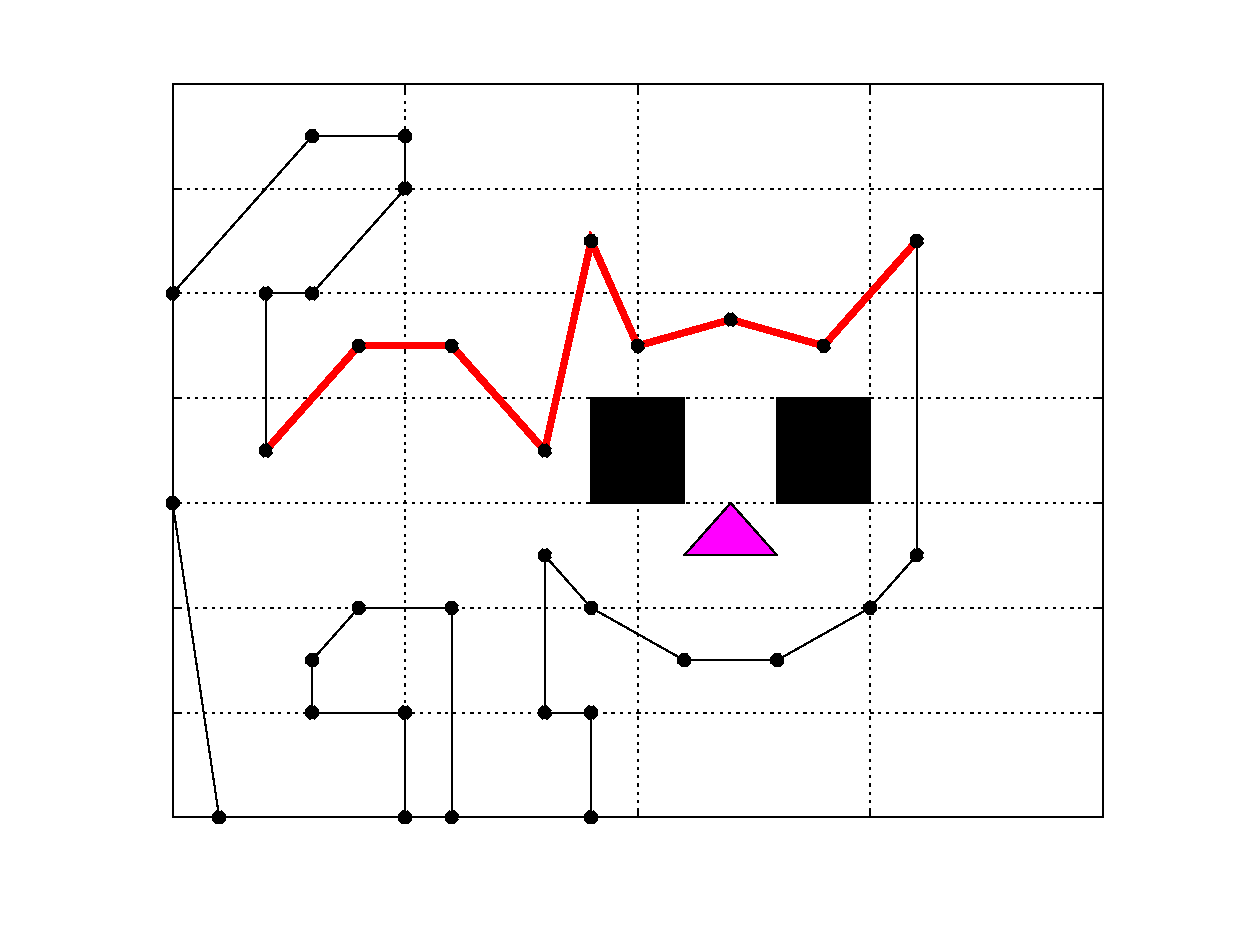
\includegraphics{gatito-inc}
\end{picture}%
\begin{picture}(576,432)(0,0)
\fontsize{10}{0}
\selectfont\put(74.88,42.5189){\makebox(0,0)[t]{\textcolor[rgb]{0,0,0}{{0}}}}
\fontsize{10}{0}
\selectfont\put(186.48,42.5189){\makebox(0,0)[t]{\textcolor[rgb]{0,0,0}{{5}}}}
\fontsize{10}{0}
\selectfont\put(298.08,42.5189){\makebox(0,0)[t]{\textcolor[rgb]{0,0,0}{{10}}}}
\fontsize{10}{0}
\selectfont\put(409.68,42.5189){\makebox(0,0)[t]{\textcolor[rgb]{0,0,0}{{15}}}}
\fontsize{10}{0}
\selectfont\put(521.28,42.5189){\makebox(0,0)[t]{\textcolor[rgb]{0,0,0}{{20}}}}
\fontsize{10}{0}
\selectfont\put(69.8755,47.52){\makebox(0,0)[r]{\textcolor[rgb]{0,0,0}{{2}}}}
\fontsize{10}{0}
\selectfont\put(69.8755,97.8171){\makebox(0,0)[r]{\textcolor[rgb]{0,0,0}{{4}}}}
\fontsize{10}{0}
\selectfont\put(69.8755,148.114){\makebox(0,0)[r]{\textcolor[rgb]{0,0,0}{{6}}}}
\fontsize{10}{0}
\selectfont\put(69.8755,198.411){\makebox(0,0)[r]{\textcolor[rgb]{0,0,0}{{8}}}}
\fontsize{10}{0}
\selectfont\put(69.8755,248.709){\makebox(0,0)[r]{\textcolor[rgb]{0,0,0}{{10}}}}
\fontsize{10}{0}
\selectfont\put(69.8755,299.006){\makebox(0,0)[r]{\textcolor[rgb]{0,0,0}{{12}}}}
\fontsize{10}{0}
\selectfont\put(69.8755,349.303){\makebox(0,0)[r]{\textcolor[rgb]{0,0,0}{{14}}}}
\fontsize{10}{0}
\selectfont\put(69.8755,399.6){\makebox(0,0)[r]{\textcolor[rgb]{0,0,0}{{16}}}}
\fontsize{10}{0}
\selectfont\put(298.08,409.6){\makebox(0,0)[b]{\textcolor[rgb]{0,0,0}{{Gatito}}}}
\end{picture}
} & \scalebox{0.42}{% Title: glps_renderer figure
% Creator: GL2PS 1.3.8, (C) 1999-2012 C. Geuzaine
% For: Octave
% CreationDate: Thu Jun 19 09:39:29 2014
\setlength{\unitlength}{1pt}
\begin{picture}(0,0)
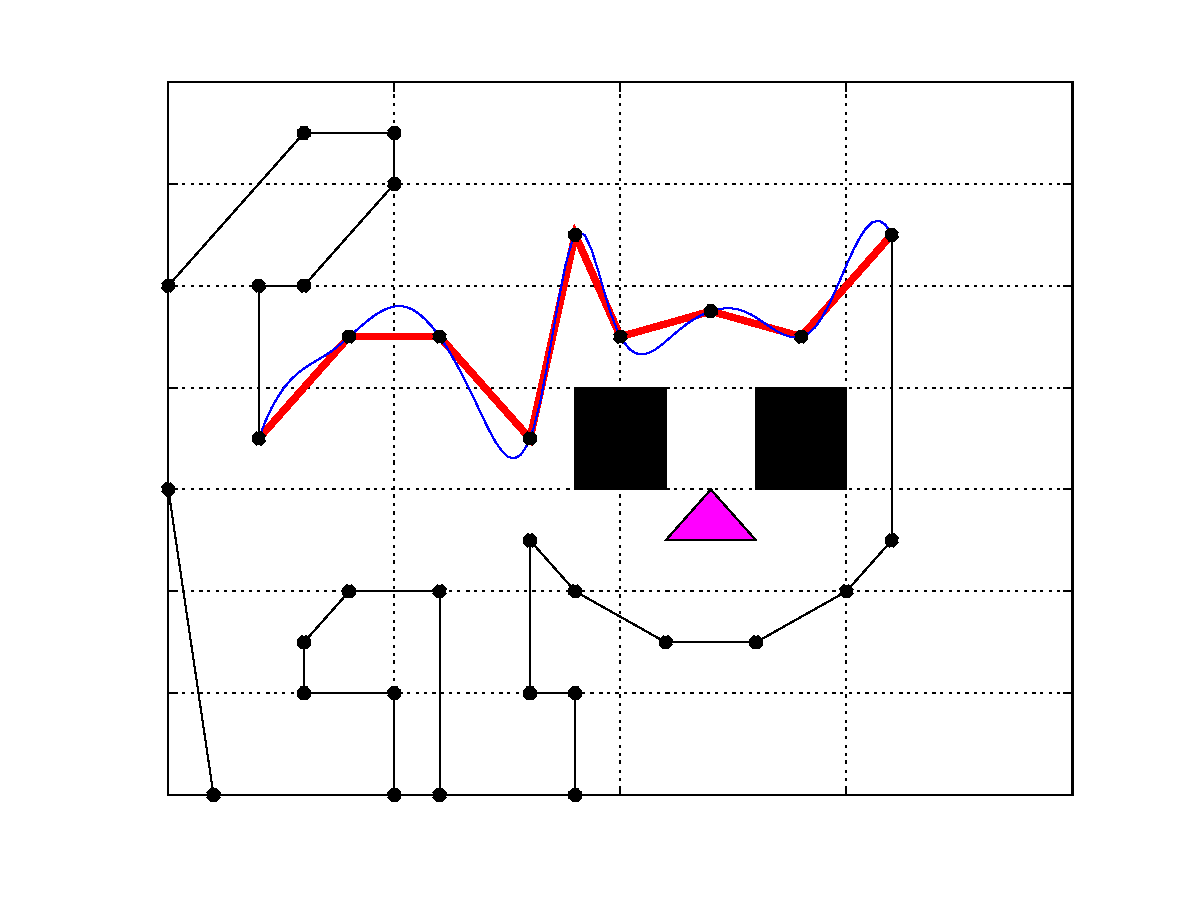
\includegraphics{gatitosplines-inc}
\end{picture}%
\begin{picture}(560,420)(0,0)
\fontsize{10}{0}
\selectfont\put(72.8,41.1956){\makebox(0,0)[t]{\textcolor[rgb]{0,0,0}{{0}}}}
\fontsize{10}{0}
\selectfont\put(181.3,41.1956){\makebox(0,0)[t]{\textcolor[rgb]{0,0,0}{{5}}}}
\fontsize{10}{0}
\selectfont\put(289.8,41.1956){\makebox(0,0)[t]{\textcolor[rgb]{0,0,0}{{10}}}}
\fontsize{10}{0}
\selectfont\put(398.3,41.1956){\makebox(0,0)[t]{\textcolor[rgb]{0,0,0}{{15}}}}
\fontsize{10}{0}
\selectfont\put(506.8,41.1956){\makebox(0,0)[t]{\textcolor[rgb]{0,0,0}{{20}}}}
\fontsize{10}{0}
\selectfont\put(67.8,46.2){\makebox(0,0)[r]{\textcolor[rgb]{0,0,0}{{2}}}}
\fontsize{10}{0}
\selectfont\put(67.8,95.1){\makebox(0,0)[r]{\textcolor[rgb]{0,0,0}{{4}}}}
\fontsize{10}{0}
\selectfont\put(67.8,144){\makebox(0,0)[r]{\textcolor[rgb]{0,0,0}{{6}}}}
\fontsize{10}{0}
\selectfont\put(67.8,192.9){\makebox(0,0)[r]{\textcolor[rgb]{0,0,0}{{8}}}}
\fontsize{10}{0}
\selectfont\put(67.8,241.8){\makebox(0,0)[r]{\textcolor[rgb]{0,0,0}{{10}}}}
\fontsize{10}{0}
\selectfont\put(67.8,290.7){\makebox(0,0)[r]{\textcolor[rgb]{0,0,0}{{12}}}}
\fontsize{10}{0}
\selectfont\put(67.8,339.6){\makebox(0,0)[r]{\textcolor[rgb]{0,0,0}{{14}}}}
\fontsize{10}{0}
\selectfont\put(67.8,388.5){\makebox(0,0)[r]{\textcolor[rgb]{0,0,0}{{16}}}}
\fontsize{10}{0}
\selectfont\put(289.8,398.5){\makebox(0,0)[b]{\textcolor[rgb]{0,0,0}{{Gatito con Splines}}}}
\end{picture}
}\\
\end{tabular}
 \end{mybox}




%\vspace{3cm}
%\noindent
%\includegraphics[width=\textwidth]{pubmm2.png}

\newpage
%%% Local Variables: 
%%% mode: latex
%%% TeX-master: "informaticaeningenieria"
%%% End: 



